\scanpage{52}
\uline{Biextensions \unsure{sous hyp. de|en hyp. de} rigidité}

$A,G$ faisceaux abéliens sur topos $S$, $f:A\longrightarrow S$
\margin{\diagram{\begin{tikzcd}[ampersand replacement=\&, column sep=small] S\arrow[r,no head]\&\text{objet final}\end{tikzcd}}}

a) Supposons $\underline{\operatorname{Hom}}_{\unsure{grs|gr}}(A,G)\simeq0$. Alors
\[
\operatorname{Ext}^1(A,G)\xrightarrow{\sim}H^0(S,\underline{\operatorname{Ext}}(A,G))
\]
donc la connaissance du \uline{faisceau} $\underline{\operatorname{Ext}}(A,G)$ implique celle de $\operatorname{Ext}(A,G)$ \unsure{et ts des} $\operatorname{Ext}(A_{\unsure{T|S}},G_{\unsure{T|S}})$.

b) Supposons $\underline{\operatorname{Hom}}_{\unsure{pct|pt}}(A,G)=0$, Alors
\margin{i.e. $f_*(G_A)\xleftarrow{\sim}G$}
\margin{\figure{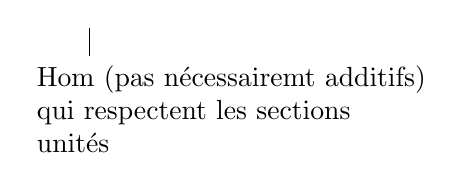
\begin{tikzpicture}\draw (0,0)--(0,-.35);\node[anchor=north,align=left] at (1.8,-.35) {\unsure{Hom (pas nécessairemt additifs)}\\qui \unsure{respectent} les sections\\unités};\end{tikzpicture}}}
\diagram{\begin{tikzcd}[ampersand replacement=\&, column sep=small,row sep=small]
H^1(A,\unsure{A_G|G_A})\simeq H^1(S,G)\times \& \underline{H^0(S,R^1f_*(G_A))}\arrow[d,phantom,"\rotatebox{90}{$\simeq$}"]\\
\&\begin{gathered}\text{Classes à isom près de $G_A$-torseurs}\\\text{\deleted{\unsure{fou}}}\ \text{rigidi\uline{fiés} rel. à $e_A$}\end{gathered}\arrow[d,phantom,"\rotatebox{90}{$\simeq$}"]\\
\&\begin{gathered}\text{Classes de \deleted{torseurs} $G_A$-torseurs}\\\text{rigidi\uline{fiables} rel. à $e_A$.}\end{gathered}
\end{tikzcd}}
\margin{\figure{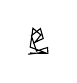
\begin{tikzpicture}[scale=.5]\draw(0,0)--(.4,.05)--(.05,.18)--(.12,.66)--(.32,.49)--(.17,.3)--(.38,.4)--(.31,.65)--(.08,.47)--(.21,.08)--(.49,.17)--(.5,.02)--(.05,.03);\end{tikzpicture}}}

De plus, le foncteur oubli, qui va de la catégorie des extensions de $A$ par $G$ en la catégorie des $G_A$-torseurs $e_A$-rigidifiés, est un fonct. pl. fid. (de catégories discrètes), (i.e. on a une \uline{injection}
\[
0\longrightarrow\operatorname{Ext}^1(A,G)\longrightarrow H^1(A,G_A)
\]
); l'image essentielle est formée des \deleted{\unsure{classes}\inserted{\unsure{fib}}} $G_A$-torseurs tels que \deleted{\unsure{classes.}\quad$\xi$\quad\unsure{telles}}
\[
\pi^*(\deleted{\unsure{F}}L)\simeq\operatorname{pr}_1^*(L)\operatorname{pr}_2(L)
\]
i.e tels que
\[
\pi^{\unsure{*|\alpha}}(L)\operatorname{pr}_1^*(L)^{-1}\operatorname{pr}_2^{\unsure{*|\alpha}}(L)^{-1}\simeq0.
\]
On trouve encore comme \unsure{corollaire} une suite exacte
\margin{\diagram{\begin{tikzcd}[ampersand replacement=\&, column sep=large]
A\times A\arrow[r,shift left=2.5ex,"\operatorname{pr}_1"]\arrow[r,"\operatorname{pr}_2"]\arrow[r,shift right=2.5ex,"\pi"']\&A
\end{tikzcd}}}
\diagram{\begin{tikzcd}[ampersand replacement=\&, column sep=small,row sep=large]
0\arrow[r,no head]\&\underline{\operatorname{Ext}}^1(A,G)\arrow[r,"i"]\&R^1f_*(G_A)\arrow[r,"j"]\arrow[d,"k"']\&\underline{\operatorname{Tors}}\ \underline{\mathrm{birig}}\ \underline{\mathrm{sym}}(A,A;G)\\
\text{i.e.}\&0\arrow[r]\&\underline{\mathrm{NS}}(A)\arrow[r,"\deleted{\unsure{k}}","j'"']\&\underline{\operatorname{Tors}}\ \underline{\mathrm{birig}}\ \underline{\mathrm{sym}}(\unsure{B|A},A;G)\arrow[u,phantom,"\unsure{\wr|i}"]\arrow[u,phantom,shift right=3ex,"\text{''}"]
\end{tikzcd}}
\margin{51}
